%%%%%%%%%%%%%%%%%%%%%%%%%%%%%%%%%%%%%%%%%%%%%%%%%%%%%%%%
\documentclass[10pt, aspectration=169]{beamer}
\usepackage[many]{tcolorbox}
% \usetheme{Copenhagen}
\usetheme{Frankfurt}
\setbeamercovered{transparent=30}
\usepackage[english]{babel}
\usepackage[utf8]{inputenc}
\usepackage{times}
\usepackage[T1]{fontenc}
\usepackage{array}
\usepackage{booktabs}
\usepackage{colortbl}
\usepackage{multirow}
\usepackage{graphicx}
\usepackage{mathrsfs}
\usepackage{bbding}
\usepackage{pifont}
\usepackage{wasysym}
\usepackage{amssymb}
\usepackage{enumerate}
\usepackage{booktabs,threeparttable}
\usepackage{adjustbox}
\usepackage{tikz}
\usetikzlibrary{calc}
% \usepackage{natbib}
\usepackage{geometry}
\geometry{papersize={160mm,100mm}, total={140mm,75mm}} % Adjust values as needed


% DEFINE COLORPALETTE
\newcommand{\cmark}{\ding{51}}%
\newcommand{\xmark}{\ding{55}}
\definecolor{unibasmintlight}{RGB}{233, 255, 253}
\definecolor{unibasmint}{RGB}{165,215,210}
\definecolor{unibasmintmid}{RGB}{30,165,165}
\definecolor{unibasanthr}{RGB}{45,55,60}
\definecolor{unibasgreydark}{RGB}{140,145,150}
\definecolor{unibasred}{RGB}{210,5,55}
\definecolor{unibaspink}{RGB}{235,130,155}
\definecolor{unibasgrey}{RGB}{190,195,200}
\definecolor{unibasmintdark}{RGB}{0,110,110} 
\definecolor{unibasblack}{RGB}{0,0,0}
\definecolor{unibaswhite}{RGB}{255,255,255}

\definecolor{scenA_table}{RGB}{245, 245, 180}
\definecolor{scenB_table}{RGB}{235, 215, 245}
\definecolor{scenC_table}{RGB}{200, 225, 240}

\definecolor{capacity_upgrade}{RGB}{64, 153, 153}
\definecolor{capacity_expansion}{RGB}{162, 216, 216}


\useinnertheme{circles}
\usefonttheme[onlymath]{serif}
\setbeamertemplate{caption}[numbered]
\usepackage{graphicx}


\newcommand{\backupbegin}{
	\newcounter{framenumberappendix}
	\setcounter{framenumberappendix}{\value{framenumber}}
}
\newcommand{\backupend}{
	\addtocounter{framenumberappendix}{-\value{framenumber}}
	\addtocounter{framenumber}{\value{framenumberappendix}} 
}

\AtBeginEnvironment{block}{%
	\setbeamercolor{itemize item}{         fg=black}
	\setbeamercolor{itemize subitem}{      fg=black}
	\setbeamercolor{itemize subsubitem}{   fg=black}
	\setbeamercolor{enumerate item}{       fg=unibasmint, bg=unibasmintdark}
	\setbeamercolor{enumerate subitem}{    fg=unibasmintdark}
	\setbeamercolor{enumerate subsubitem}{ fg=unibasmintdark}
	\setbeamercolor{item projected}{       fg=white, bg=unibasmintdark}
}

\AtBeginEnvironment{alertblock}{%
    \setbeamercolor{itemize item}{fg=      black}
    \setbeamercolor{itemize subitem}{      fg=black}
	\setbeamercolor{itemize subsubitem}{   fg=black}
	\setbeamercolor{enumerate item}{       fg=unibasmint, bg=red}
	\setbeamercolor{enumerate subitem}{    fg=unibasmintdark}
	\setbeamercolor{enumerate subsubitem}{ fg=unibasmintdark}
	\setbeamercolor{item projected}{       fg=white, bg=unibasmintdark}
}


% SET CITATION
%\usepackage[backend = biber, style = apa, maxbibnames=999, minbibnames = 1, maxcitenames=2, mincitenames=1, uniquelist=true]{biblatex}
\usepackage[backend = biber, style = apa, maxbibnames=999, minbibnames = 1, maxcitenames=1, mincitenames=1, uniquelist=true]{biblatex}

\addbibresource{sured.bib}
\AtBeginBibliography{\small}
\hypersetup{colorlinks = true, 
            citecolor = unibasmintmid, 
            linkcolor = white, 
            urlcolor = unibasmintdark}

% % SET BEAMER COLOR
\setbeamercolor*{structure}{                        fg=unibasmint,bg=unibasblack}
\setbeamercolor*{palette primary}{use=structure,    fg=unibasblack,bg=structure.fg}
\setbeamercolor*{palette secondary}{use=structure,  fg=white,bg=structure.fg!75!black}
\setbeamercolor*{palette tertiary}{use=structure,   fg=white,bg=structure.fg!50!black}
\setbeamercolor*{palette quaternary}{               fg=black,bg=white}
\setbeamercolor*{item projected}{                   fg=black,bg=unibasmint!80}
\setbeamercolor*{block title example}{              fg=black,bg=unibasmint}
\setbeamercolor{title}{bg=white,                    fg=unibasmintdark}

\setbeamercolor{button}{bg=unibasmint,fg=black}
\setbeamercolor{section in toc}{fg=unibasmintdark,bg=white} %Here we adjust colors for table of contents
\setbeamercolor{subsection in toc}{fg=unibasgreydark,bg=white}
\setbeamercolor{block title}{bg=unibasmintdark,fg=unibasmint}  %Here I changed color of the block! See Slide 3
\setbeamercolor{itemize item}{fg=black}
\setbeamercolor{itemize subitem}{fg=black}
\setbeamercolor{itemize subsubitem}{fg=unibasmintdark}
\setbeamercolor{frametitle}{bg=unibasmintlight,fg=unibasmintdark}


\setbeamertemplate{blocks}[rounded][shadow=false] %Here I make bullet points as circles; Here I make rounded blocks with shadow
\setbeamertemplate{itemize item}[circle]
\setbeamertemplate{itemize subitem}{$-$}
\setbeamertemplate{itemize subsubitem}[triangle]

% SET TITLEPAGE LAYOUT
\setbeamertemplate{title page}
{
    \begin{beamercolorbox}[sep=8pt,center,shadow=false,rounded=false]{title}
        \usebeamerfont{title}\inserttitle\par%
        \ifx\insertsubtitle\@empty%
        \else%
            \vskip0.25em%
            {\usebeamerfont{subtitle}\usebeamercolor[fg]{subtitle}\insertsubtitle\par}%
        \fi%     
    \end{beamercolorbox}%
    \vskip1em\par
    \begin{beamercolorbox}[sep=8pt,center]{author}
        \usebeamerfont{author}\insertauthor
    \end{beamercolorbox}
    \begin{beamercolorbox}[sep=8pt,center]{institute}
        \usebeamerfont{institute}\insertinstitute
    \end{beamercolorbox}
    \begin{beamercolorbox}[sep=8pt,center]{date}
        \usebeamerfont{date}\insertdate
    \end{beamercolorbox}
}


% shift all titles per slide a bit downwords
\makeatletter
\setbeamertemplate{frametitle}{
  \vspace{0.12cm}% Increase this value as needed
  \insertframetitle
}
\makeatother  

% background title per slide


% navigation bar
\useoutertheme{infolines}      
\setbeamertemplate{headline}[default]
\setbeamertemplate{navigation symbols}{}
\useoutertheme[subsection=false]{miniframes}

% color footer
\setbeamercolor{author in head/foot}{fg=white,      bg=unibasmintdark}
\setbeamercolor{title in head/foot}{fg=white,       bg=unibasmintdark}
\setbeamercolor{date in head/foot}{fg=white,        bg=unibasmintdark}
\setbeamercolor{section in head/foot}{fg=white,     bg=unibasmintdark}
\setbeamercolor{subsection in head/foot}{fg=white,  bg=unibasmintdark}
% \setbeamercolor{author in head/foot}{fg=black,      bg=unibasmint}
% \setbeamercolor{title in head/foot}{fg=black,       bg=unibasmint}
% \setbeamercolor{date in head/foot}{fg=black,        bg=unibasmint}
% \setbeamercolor{section in head/foot}{fg=black,     bg=unibasmint}
% \setbeamercolor{subsection in head/foot}{fg=black,  bg=unibasmint}
% \setbeamercolor*{palette primary}{fg=black,   bg=unibasmint}
% \setbeamercolor*{palette secondary}{fg=black, bg=unibasmint}
% \setbeamercolor*{palette tertiary}{fg=black,  bg=unibasmint}
% \setbeamercolor*{palette quaternary}{fg=black,bg=unibasmint}


% Title page %***************************************************************
\title[Improved Residential PV Expansion]{Decisions at the Grid's Edge: \\ An Improved Spatial PV Expansion in Swiss Residences}

\author{Raul Hochuli}
\institute[University of Basel]{University of Basel, Faculty of Business and Economics, } 
\date[June 2026]{June 2026}
\titlegraphic{\includegraphics[width=2.3cm]{UniBas_Logo.jpg}}



%*******************************************************************************
\begin{document}  %%%%%%%%%%%%%%%%%%%%%%%%%%%%%%%%%%%%%%%%%%%%%%%
%******************************************************************************

% =======================================
\begin{frame}
    \maketitle
\end{frame}


%%%%%%%%%%%%%%%%%%%%%%%%%%%%%%%%%%%%%%%%%%%%%%%
\section{Motivation \& Literature} 

% =======================================
\begin{frame}{}
  \centering
  \makebox[0pt][c]{%
    
\includegraphics[width=0.9841\textwidth]{paper_publication/SURED_Ascona/figures/newspaper_header3.png}
  }

% https://www.iea.org/reports/global-energy-review-2026/technology-solar-pv-and-wind
% https://www.bloomberg.com/news/newsletters/2025-10-28/europe-s-solar-power-surge-puts-unprecedented-strain-on-its-grid
% https://www.bloomberg.com/news/articles/2025-11-30/eon-ceo-urges-germany-to-slow-wind-solar-push-amid-grid-strain


% \href{https://www.nzz.ch/schweiz/der-solarboom-bringt-das-stromnetz-an-den-anschlag-ld.1728398}{https://www.nzz.ch/schweiz/der-solarboom-bringt-das-stromnetz-an-den-anschlag-ld.1728398}
% \href{https://www.nzz.ch/wirtschaft/die-deutsche-energiewende-geht-voran-jetzt-will-katharina-reiche-die-spielregeln-aendern-ld.1930553}{https://www.nzz.ch/wirtschaft/die-deutsche-energiewende-geht-voran-jetzt-will-katharina-reiche-die-spielregeln-aendern-ld.1930553}
% \href{https://www.spiegel.de/wirtschaft/soziales/katherina-reiche-wirtschaftsministerin-plant-massive-einschnitte-fuer-erneuerbare-energien-a-c8d3fb96-2d80-41c4-9ff4-dc7a82f9019e}{https://www.spiegel.de/wirtschaft/soziales/katherina-reiche-wirtschaftsministerin-plant-massive-einschnitte-fuer-erneuerbare-energien-a-c8d3fb96-2d80-41c4-9ff4-dc7a82f9019e}
% \href{https://www.sueddeutsche.de/wirtschaft/erneuerbare-energien-solarbranche-ausbau-erneuerbarer-energien-ist-buergerwille-dpa.urn-newsml-dpa-com-20090101-260404-930-907053}{https://www.sueddeutsche.de/wirtschaft/erneuerbare-energien-solarbranche-ausbau-erneuerbarer-energien-ist-buergerwille-dpa.urn-newsml-dpa-com-20090101-260404-930-907053}
% https://www.pilotonline.com/2026/04/21/renewable-energies-global-electricity-demand/
% https://www.nytimes.com/2013/11/11/business/energy-environment/solar-power-begins-to-shine-as-environmental-benefits-pay-off.html
\begin{block}{Research Contribution}
    \begin{enumerate}
        \item \textbf{Problem quantification}: 
        \begin{itemize}
            % \item Create highly detailed spatial model to estimate PV-induced effects in larger LV grid (incl. roof specifics + individual "decision making").
            %(incl. roof specifics production profiles + individual "decision making").
            \item \textcolor{black}{\textit{Find a data based model simulation that estimates how soon and when solar PV expansion causes "grid-problems".}}
        \end{itemize}
        \vspace{0.1cm}
        \item \textbf{Economic response}: 
        \begin{itemize}
            % \item \textcolor{unibasgreydark}{1st-best) Congestion pricing for externality (not feasible in practice)}
            % \item 2nd-best) Simple subsidy adjustments, focusing on grid capacity
            \item \textcolor{black}{\textit{2nd-best solution: Simple subsidy adjustments might delay grid congestion for a more efficient outcome. }}
        \end{itemize}
    \item \textbf{Not included}: 
        \begin{itemize}
            % \item \textcolor{unibasgreydark}{1st-best) Congestion pricing for externality (not feasible in practice)}
            % \item 2nd-best) Simple subsidy adjustments, focusing on grid capacity
            \item \textcolor{black}{\textit{Local battery storage is not included in the simulation, but considered in the post-analysis}}
        \end{itemize}


    \end{enumerate}
\end{block}

\end{frame}

% =======================================
\begin{frame}{About PV...}
\centering
\definecolor{card1}{RGB}{165,200,220}
\definecolor{card2}{RGB}{125,165,190}
\definecolor{card3}{RGB}{90,130,160}
\definecolor{card4}{RGB}{55,95,130}
\definecolor{card5}{RGB}{25,60,95}
\definecolor{card6}{RGB}{0,25,60}
\definecolor{bottomcard}{RGB}{45,55,60}

\begin{tikzpicture}[scale=0.95, transform shape, xshift=-0.8cm]
\newcommand{\cardwidth}{2.0cm}
\tikzset{
  topiccard/.style={
    rounded corners=6pt,
    minimum width=2.4cm,
    minimum height=3.0cm,
    align=left,
    text=white,
    font=\small
  },
  smallcard/.style={
    rounded corners=6pt,
    minimum width=2.4cm,
    minimum height=0.9cm,
    align=left,
    text=white,
    font=\small
  }
}

% =====================================================
% MAIN ROW — 4 cards side by side at y=0
% =====================================================

\node[topiccard, fill=card3, ] (t1) at (0, 0)
{
\begin{minipage}{\cardwidth}
\raggedright
{\bfseries Goals \& Scenarios}\\
\vspace{0.1cm}
\scriptsize
37.5 GW by 2050 \hyperlink{appendix_res_targets}{\beamerreturnbutton{\tiny{Targets}}}\\
\hfill{\tiny\cite{bfe_ep2050_2020}}
\end{minipage}
};


\node[topiccard, fill=card4, fill opacity=0.35, text opacity=0.95 ] (t2) at (2.5, 0)
{
\begin{minipage}{\cardwidth}
\raggedright
{\bfseries Grid Cost Estimates}\\
\vspace{0.1cm}
\scriptsize
LV: CHF 600m pa until 2050\\
\hfill{\tiny\cite{bfe_ep2050_netz2022}}\\
\vspace{0.05cm}
Poss. underestimation \hyperlink{appendix_model_grid_analysis}{\beamerreturnbutton{\tiny{Grid Analysis}}}
\end{minipage}
};

\node[topiccard, fill=card5, fill opacity=0.35, text opacity=0.95] (t3) at (5.0, 0)
{
\begin{minipage}{\cardwidth}
\raggedright
{\bfseries Drivers \& Acceptance}\\
\vspace{0.1cm}
\scriptsize
Key Factors\\
\hfill{\tiny\cite{muller2020}}\\
\vspace{0.05cm}
Reluctance\\
\hfill{\tiny\cite{sutterlin2017, cousse2020}}
\end{minipage}
};

\node[topiccard, fill=card6] (t4) at (7.5, 0)
{
\begin{minipage}{\cardwidth}
\raggedright
{\bfseries Future / Optimal Inst.}\\
\vspace{0.1cm}
\scriptsize
NPV Proxy\\
\hfill{\tiny\cite{arguello2018}}\\
\vspace{0.05cm}
MV grid\\
\hfill{\tiny\cite{gupta2021}}\\
\vspace{0.05cm}
Biodiversity a.o.\\
\hfill{\tiny\cite{hermoso2023}}
\end{minipage}
};

% =====================================================
% STACKED PAIR — Grid Effects (top) + Smart Meters (bottom)
% =====================================================

\node[smallcard, fill=card2, fill opacity=0.35, text opacity=0.95] (s1) at (10.3, 0.75)
{
\begin{minipage}{\cardwidth}
\raggedright
{\bfseries Grid Effects}\\
\vspace{0.05cm}
\scriptsize
Penetration limits\\
\hfill{\tiny\cite{tevar2019}}
\end{minipage}
};

\node[smallcard, fill=card2, fill opacity=0.35, text opacity=0.95] (s2) at (10.3, -0.75)
{
\begin{minipage}{\cardwidth}
\raggedright
{\bfseries Smart Meters}\\
\vspace{0.05cm}
\scriptsize
Rollout 2028 at 80\%\\
\hfill{\tiny\cite{elcom_smartmeter_2026}}
\end{minipage}
};

% =====================================================
% BOTTOM SUMMARY CARD
% =====================================================

\node[
  rounded corners=8pt,
  fill=bottomcard,
  minimum width=12.7cm,
  minimum height=0.75cm,
  text=white,
  align=center
] (bottom) at (5.15, -2.1)
{
  Increasing PV deployment outpaces grid infrastructure (globally).
};

% =====================================================
% CONNECTION LINES
% =====================================================

\foreach \n in {t1,t2,t3,t4}
{
  \draw[gray!60, thick]
  (\n.south) -- (\n.south |- bottom.north);
}

% s2 — straight down
\draw[gray!60, thick]
  (s2.south) -- (s2.south |- bottom.north);

% s1 — jog right before going down, so it clears s2
\draw[gray!60, thick]
  (s1.south)
  -- ($(s1.south) + (0, -0.25)$)           % step down just below s1
  -- ($(s1.south) + (0.45, -0.25)$)        % step right past s2 edge
  -- ($(s1.south) + (0.45, -0.25)$  |- bottom.north); % down to bottom bar
  
\end{tikzpicture}

\vspace{0.3cm}
\makebox[0pt][c]{%
  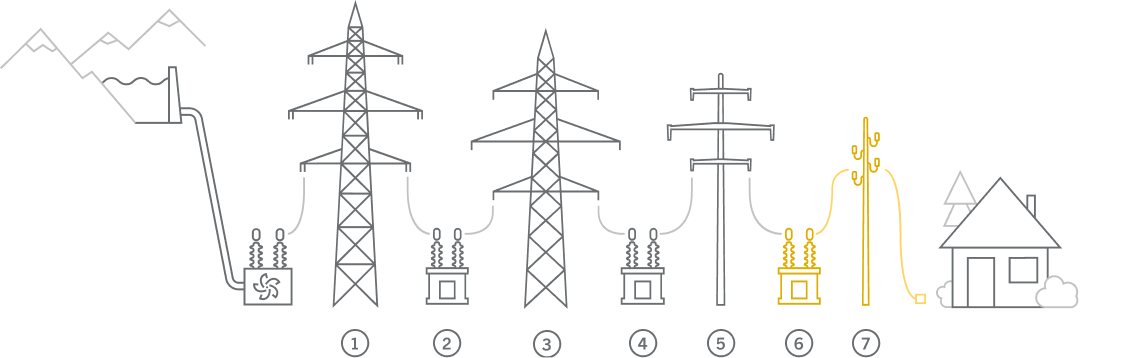
\includegraphics[width=0.81\textwidth]{figures/grid-levels.png}
}

\end{frame}


%%%%%%%%%%%%%%%%%%%%%%%%%%%%%%%%%%%%%%%%%%%%%%%
\section{Model} 

% =======================================
\begin{frame}{Model Simulation - 3 Agents }
\hypertarget{mod_structure_agents}{}

\begin{columns}[t]
    % \begin{column}{0.49\textwidth}    
    % \only<1->{\textcolor[RGB]{128, 0, 128}{Production}
    % \begin{itemize}
    %     \item Roof partitions and radiation yield production potential.
    %     \item Calibrated random forest assigns installation size \hyperlink{appendix_randomforest_scatterplot}{\beamerreturnbutton{App. RFR}}.
    % \end{itemize}}

    % \only<2->{\textcolor[RGB]{204, 85, 0}{Demand} ($\rightarrow$ \textcolor[RGB]{0, 70, 127}{Feed-in})
    % \begin{itemize}
    %     \item 6 Archetype profiles scaled by living area (\cite{swissstore2022}). 
    %     \item Scaling up winter months for houses with heat pumps.
    % \end{itemize}}

    % \only<3->{\textcolor{unibasgreydark}{Investments}
    % \begin{itemize}
    %     \item General cost assumption of PV calculator (\cite{energieschweiz2023} \hyperlink{appendix_cost_function}{\beamerreturnbutton{App. Cost}})
    % \end{itemize}
    % \vspace{0.1875cm}
    % $\rightarrow NPV_{i} = -Inv_{i} + \sum_{t}^{25}\frac{SelfCons_{i,t} P_{elec,t} + Feedin_{i,t} P_{pv,t} }{(1+r)^t}$}
    % \end{column}
    
    % \begin{column}{0.49\textwidth}    
    %     % Top figure: always visible
    %     \begin{figure}
    %         \centering
    %         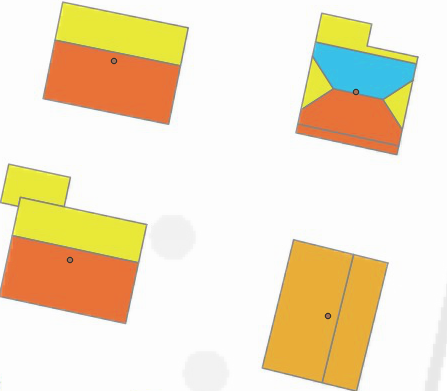
\includegraphics[width=0.481\linewidth]{figures/EGID_solkat_example.png}
    %         \label{fig:placeholder}
    %     \end{figure}
    %     % Bottom figure: swaps with each step
    %     \begin{figure}
    %         \centering
    %         \only<1>{
\includegraphics[width=0.91\linewidth]{figures/plot_EGID_HOY_pvprod.png}}
    %         \only<2>{
\includegraphics[width=0.91\linewidth]{figures/plot_EGID_HOY_pvprod_demand.png}}
    %         \only<3>{
\includegraphics[width=0.91\linewidth]{figures/plot_EGID_HOY_pvprod_demand_feedin.png}}
    %         \label{fig:placeholder}
    %     \end{figure}
    % \end{column}
\begin{column}{0.49\textwidth}
    \only<1->{\textcolor[RGB]{128, 0, 128}{Production}
    \begin{itemize}
        \item Roof partitions and radiation time series yield production potential.
        \item Calibrated random forest assigns installation size \hyperlink{appendix_randomforest_scatterplot}{\beamerreturnbutton{App. RFR}}.
    \end{itemize}}
    \only<2->{\textcolor[RGB]{204, 85, 0}{Demand} ($\rightarrow$ \textcolor[RGB]{0, 70, 127}{Feed-in})
    \begin{itemize}
        \item 6 Archetype profiles scaled by living area (\cite{swissstore2022}).
        \item Scaling up winter months for houses with heat pumps.
    \end{itemize}}
    \only<3->{\textcolor{unibasgreydark}{Investments}
    \begin{itemize}
        \item General cost assumption of PV calculator (\cite{energieschweiz2023} \hyperlink{appendix_cost_function}{\beamerreturnbutton{App. Cost}})
    \end{itemize}
    \vspace{0.1875cm}
    $\rightarrow NPV_{i} = -Inv_{i} + \sum_{t}^{25}\frac{SelfCons_{i,t} P_{elec,t} + Feedin_{i,t} P_{pv,t} }{(1+r)^t}$}
    \vfill % Push all content to the top
\end{column}

\begin{column}{0.49\textwidth}    
    % Top figure: always visible
    \begin{figure}
        \centering
        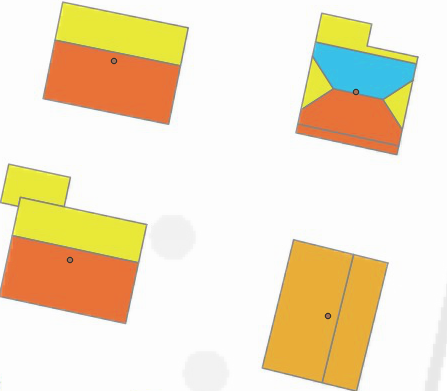
\includegraphics[width=0.481\linewidth]{figures/EGID_solkat_example.png}
        \label{fig:placeholder}
    \end{figure}
    % Bottom figure: swaps with each step
    \begin{figure}
        \centering
        \only<1>{
\includegraphics[width=0.91\linewidth]{figures/plot_EGID_HOY_pvprod.png}}
        \only<2>{
\includegraphics[width=0.91\linewidth]{figures/plot_EGID_HOY_pvprod_demand.png}}
        \only<3>{
\includegraphics[width=0.91\linewidth]{figures/plot_EGID_HOY_pvprod_demand_feedin.png}}
        \label{fig:placeholder}
    \end{figure}
\end{column}

\end{columns}
\end{frame}

% =====================================================
\begin{frame}{Allocation Process}
\hypertarget{mod_allocation_process}{}
\begin{columns}[t]

% LEFT COLUMN
\begin{column}{0.49\textwidth}

\textbf{Allocation process}

\begin{itemize}
    % \item Installation "order" defined by NPV.
    \item NPV defines installation "order" (similar to \cite{arguello2018}, \hyperlink{appendix_npv_hist_sensitivity}{\beamerreturnbutton{App. NPV sensitivity}}).
    \item Scaled, adujsted, annual "construction budget" (\cite{bfe_ep2050_2020}) until 2050.
\end{itemize}

\vspace{-0.2cm}

\begin{figure}
    \centering
    \includegraphics[width=0.84\linewidth]{figures/pvalloc_LRG3_max_npv_df_hist.png}
\end{figure}

\end{column}


% RIGHT COLUMN
\begin{column}{0.49\textwidth}

\textbf{Subsidy adjustment}

\begin{itemize}
    \item Subsidy budget given to operator (transparent criteria)
    \item 3 types (A: roof orientation, B: grid specific, C: combination)
\end{itemize}

% \vspace{0.3cm}

% \textbf{Decision rule}

\[
\rightarrow NPV_{i,X} = NPV_{i} + S_{i,X} - R_{i,X}
\]

\vspace{0.3cm}

\centering
\footnotesize
\begin{tabular}{|l| c c c c|}
    \hline
    & $S=0$ & 4000 & 6000 & 8000 \\
    \hline
    $R=0$    & BU & \cellcolor{scenA_table} & \cellcolor{scenA_table} A & \cellcolor{scenA_table} \\
    4000     & \cellcolor{scenB_table} & \cellcolor{scenC_table} & \cellcolor{scenC_table} & \cellcolor{scenC_table} \\
    6000     & \cellcolor{scenB_table} B & \cellcolor{scenC_table} & \cellcolor{scenC_table} C & \cellcolor{scenC_table} \\
    8000     & \cellcolor{scenB_table} & \cellcolor{scenC_table} & \cellcolor{scenC_table} & \cellcolor{scenC_table} \\
    \hline
\end{tabular}

\end{column}

\end{columns}
\end{frame}

%%%%%%%%%%%%%%%%%%%%%%%%%%%%%%%%%%%%%%%%%%%%%%%
\section{Data} 



% =======================================
\begin{frame}{Data}


% ----------- Summary Table -----------
\centering
\textbf{Summary}\\
\vspace{0.2cm}

{\scriptsize
\setlength{\tabcolsep}{3.5pt}
\renewcommand{\arraystretch}{1.15}

\begin{tabular}{|l c  c c |}
    \hline
    \textbf{Summary}      & \textbf{Sample}     & \textbf{Avail.Sample}        & \textbf{All CH} \\
    \hline
    n Municipalities        & 28    & 79        & 2'133    \\
    n All Buildings         & 44'354            & 132'018              & 3'090'962    \\
    n Resid. Houses         & 21'599             & 47'900               & 1'716'194    \\
    n Grid Nodes            & 391        & 1'113            & -    \\
    Inst. Capacity 2024 (MW) & 20.6  & 79.0    & 2'450.1 \\
    Capacity 2050 (MW)       & 115.6  & 739.5    & 17'313.8    \\
    \hline       
\end{tabular}

}

\vspace{0.6cm}

% ----------- Data Sources Table -----------
\centering
\textbf{Data Sources}\\
\vspace{0.2cm}

{\scriptsize
\setlength{\tabcolsep}{3.5pt}
\renewcommand{\arraystretch}{1.15}

\begin{tabular}{|l l l|} %p{1cm}|}
    \hline
    \textbf{Category} & \textbf{Description} & \textbf{Ref.} \\
    \hline
    Rooftop Data 
        & Roof surface, orientation, tilt
        & [1] \\
        
    Building Data 
        & Building type, heating tech, existing inst.  prices / tariffs
        & [2--5] \\
                
    Grid Infrastructure 
        & Nodes, connections + capacity
        & (NDA) \\
        
    Other Data
        & Demand, costs assumptions, capacity targets, radiation
        & [6--9] \\
        
    Computing Infrastructure
        & High Performance Cluster for model run
        & [10] \\
    \hline
\end{tabular}

\vspace{0.2cm}
}

\vspace{0.2cm}
{\tiny
\begin{minipage}{\linewidth}
\raggedright
[1]: \cite{solkat2023}\par
[2--5]: \cite{gwr2025, elec_prod2024, vese_pvtarif2023, elcom2023}\par
[6--9]: \cite{swissstore2022,  energieschweiz2023, bfe_ep2050_2020, meteoblue2023}\par
[10]: \cite{hpc_scicore2026}\par
\end{minipage}

}\end{frame}



%%%%%%%%%%%%%%%%%%%%%%%%%%%%%%%%%%%%%%%%%%%%%%%
\section{Results} 

% =======================================
\begin{frame}{\strut PV-Induced Excess Feedin}

\begin{minipage}{0.322\textwidth}
  \centering
  \makebox[0pt][c]{%
    
\includegraphics[width=\textwidth]{figures/gridnode_feedin_threshold_HOY.png}
  }
\end{minipage}\hfill
\begin{minipage}{0.322\textwidth}
  \centering
  \makebox[0pt][c]{%
    
\includegraphics[width=\textwidth]{figures/line_PVproduction_bau_excfeedin.png}
  }
\end{minipage}\hfill
\begin{minipage}{0.322\textwidth}
  \centering
  \makebox[0pt][c]{%
    
\includegraphics[width=\textwidth]{figures/line_PVproduction_bau_feedin.png}
  }
\end{minipage}
\end{frame}

% =======================================
\begin{frame}{\strut Different Subsidies}
\begin{minipage}{0.48\textwidth}
  \centering
  \makebox[0pt][c]{%
    
\includegraphics[width=\textwidth]{figures/line_PVproduction_bauABC_excfeedin.png}
  }
\end{minipage}\hfill
\begin{minipage}{0.48\textwidth}
  \centering
  \makebox[0pt][c]{%
    
\includegraphics[width=\textwidth]{figures/line_PVproduction_bauABC_feedin.png}
  }
\end{minipage}
\end{frame}

% =======================================
\begin{frame}{\strut Grid Optimal Expansion}
\begin{minipage}{0.48\textwidth}
  \centering
  \makebox[0pt][c]{%
    
\includegraphics[width=\textwidth]{figures/line_PVproduction_gridoptim_excfeedin.png}
  }
\end{minipage}\hfill
\begin{minipage}{0.48\textwidth}
  \centering
  \makebox[0pt][c]{%
    
\includegraphics[width=\textwidth]{figures/line_PVproduction_gridoptim_feedin.png}
  }
\end{minipage}
\end{frame}




%%%%%%%%%%%%%%%%%%%%%%%%%%%%%%%%%%%%%%%%%%%%%%%
\section{Outlook} 

% =======================================
\begin{frame}{Conclusion}
% \textbf{Summary}
\begin{block}{Research Contribution}
    \begin{enumerate}
        \item \textbf{Problem quantification}: 
        \begin{itemize}
            % \item Create highly detailed spatial model to estimate PV-induced effects in larger LV grid (incl. roof specifics + individual "decision making").
            %(incl. roof specifics production profiles + individual "decision making").
            \item \textcolor{black}{\textit{Problems will arise in the next couple of years might scale up fast, dependent on the growth rate of newly installed capacity.}}
        \end{itemize}
        \vspace{0.1cm}
        \item \textbf{Economic response}: 
        \begin{itemize}
            % \item \textcolor{unibasgreydark}{1st-best) Congestion pricing for externality (not feasible in practice)}
            % \item 2nd-best) Simple subsidy adjustments, focusing on grid capacity
            \item \textcolor{black}{\textit{Simple subsidy adjustments might delay grid congestion by a few years and overall size and could be even as good as a social planner's allocation. }}
        \end{itemize}
    \end{enumerate}
\end{block}

\textbf{Outlook}
\begin{itemize}
    % \item Comparison to "optimal installation schedule" (*in progress)
    % \item Allow for peak-shaving by grid operator
    % \item Use RTP instead of TOU prices for electricity self consumption.
    \item Cost comparison of subsidy spending / savings to grid reinforcements in most affected nodes.
    \item Post calculation for battery capacity for "worst week" in "worst node". 
    % \item Recalibrate future construction capacity (*in progress)
\end{itemize}

\textbf{Postponed}
\begin{itemize}
    \item Add battery investment and battery usage to the model 
    \begin{itemize}
        \item Optimized for household consumption vs. grid serving (quasi-obligatory for a PV installations)
    \end{itemize}
    % \item  More sophisticated pricing schemes (actual congestion pricing)
\end{itemize}

\end{frame}


%%%%%%%%%%%%%%%%%%%%%%%%%%%%%%%%%%%%%%%%%%%%%%%
% \section{References}


% \renewcommand{\bibfont}{\normalsize}

%%%%%%%%%%%%%%%%%%%%%%%%%%%%%%%%%%%%%%%%%%%%%%
\section*{Appendix} 

% =======================================
\begin{frame}{\strut Appendix: DSO Intervention }
\begin{minipage}{0.48\textwidth}
  \centering
  \makebox[0pt][c]{%
    
\includegraphics[width=\textwidth]{figures/line_PVproduction_DSOreact_excfeedin.png}
  }
\end{minipage}\hfill
\begin{minipage}{0.48\textwidth}
  \centering
  \makebox[0pt][c]{%
    
\includegraphics[width=\textwidth]{figures/line_PVproduction_DSOreact_feedin.png}
  }
\end{minipage}
\end{frame}

% =======================================
\begin{frame}{\strut Appendix: NPVs Sensitivity -  Electricity Prices }
\hypertarget{appendix_npv_hist_sensitivity}{}
\begin{minipage}{0.48\textwidth}
  \centering
  \makebox[0pt][c]{%
    \includegraphics[width=\textwidth]{figures/pvalloc_LRG3_max_elecpri15RP_npv_df_hist.png}
  }
\end{minipage}\hfill
\begin{minipage}{0.48\textwidth}
  \centering
  \makebox[0pt][c]{%
    \includegraphics[width=\textwidth]{figures/pvalloc_LRG3_max_elecpri60RP_npv_df_hist.png}
  }
\end{minipage}
\centering
\hyperlink{mod_allocation_process}{\beamerreturnbutton{back}}
\end{frame}

% =======================================
\begin{frame}{Appendix: High Spatial Resolution At Large Scale }
\begin{minipage}{0.323\textwidth}
  \centering
  \makebox[0pt][c]{%
    
\includegraphics[width=\textwidth]{figures/wp_topo_roof_solkat_1_3.png}
  }
\end{minipage}\hfill
\begin{minipage}{0.323\textwidth}
  \centering
  \makebox[0pt][c]{%
    
\includegraphics[width=\textwidth]{figures/wp_topo_DSO_example_1_3.png}
  }
\end{minipage}
\begin{minipage}{0.323\textwidth}
  \centering
  \makebox[0pt][c]{%
    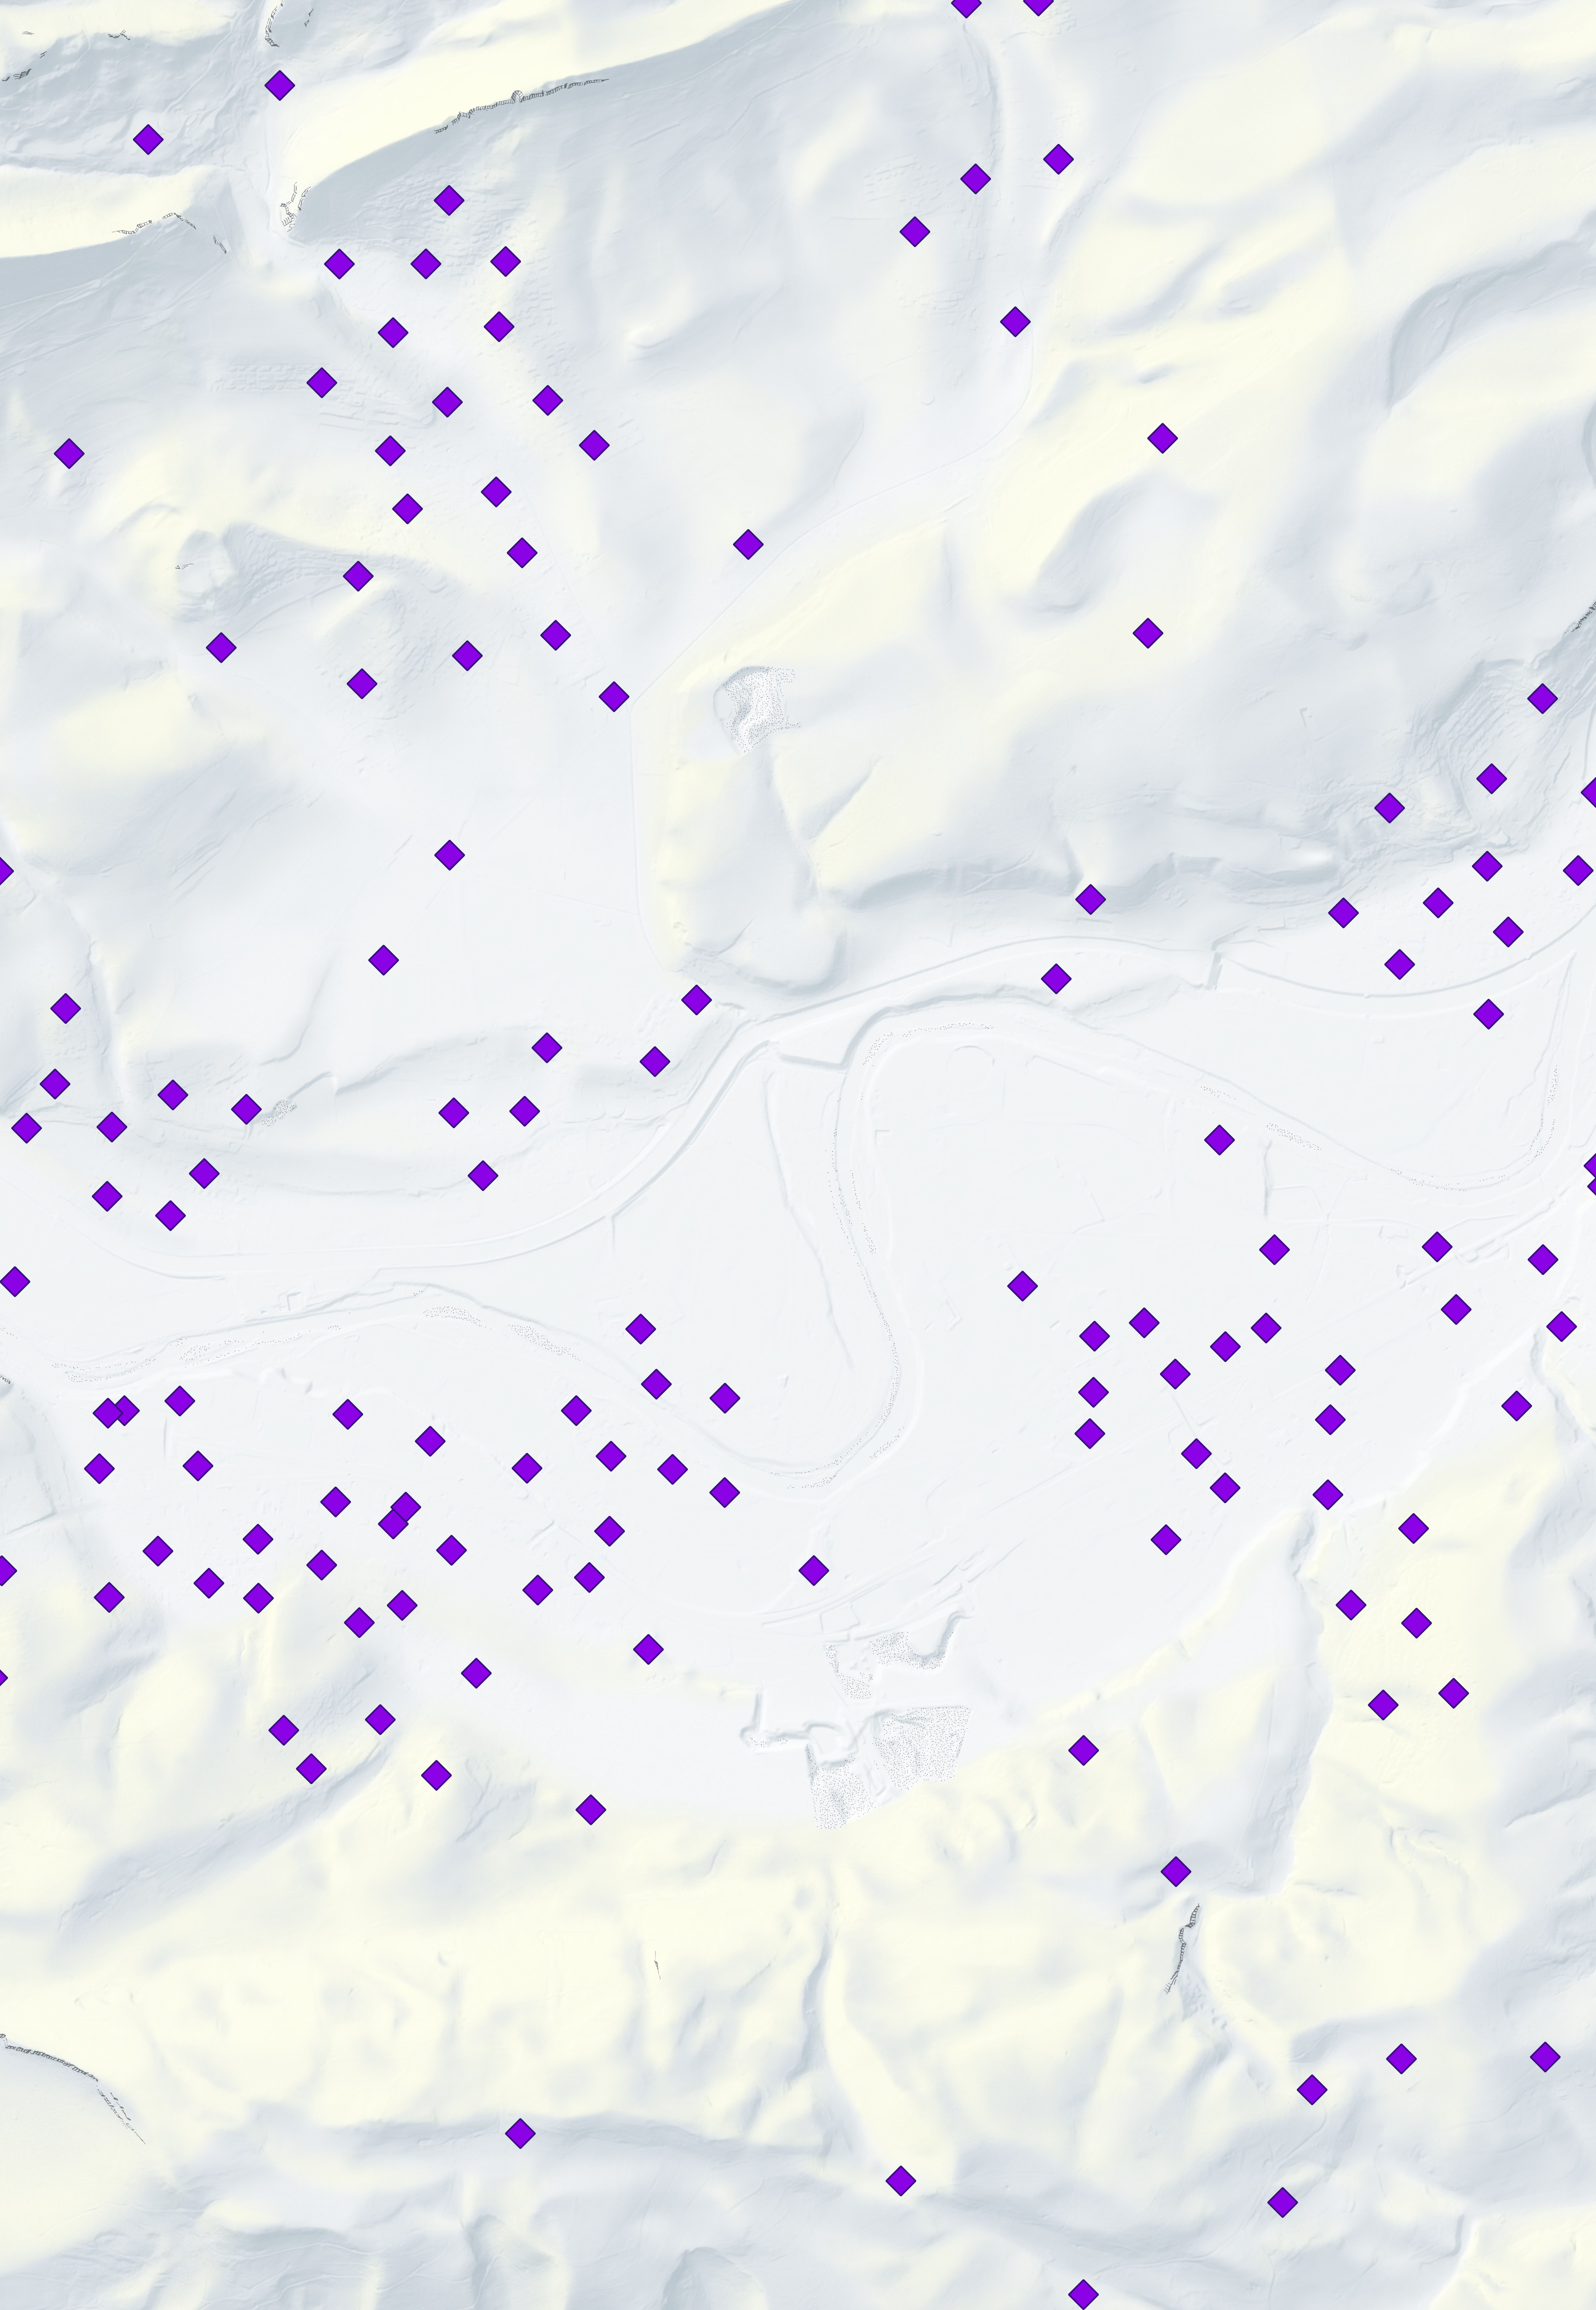
\includegraphics[width=\textwidth]{figures/wp_topo_DSO_grid_large_example_1_3.png}
  }
\end{minipage}
\end{frame}

% % =======================================
% \begin{frame}{\strut PV-Induced Excess Feedin}

% \begin{minipage}{0.322\textwidth}
%   \centering
%   \makebox[0pt][c]{%
%     
\includegraphics[width=\textwidth]{figures/NPVhist_LRG3_max_15Rp.png}
%   }
% \end{minipage}\hfill
% \begin{minipage}{0.322\textwidth}
%   \centering
%   \makebox[0pt][c]{%
%     
\includegraphics[width=\textwidth]{figures/NPVhist_LRG3_max_31Rp.png}
%   }
% \end{minipage}\hfill
% \begin{minipage}{0.322\textwidth}
%   \centering
%   \makebox[0pt][c]{%
%     
\includegraphics[width=\textwidth]{figures/NPVhist_LRG3_max_60Rp.png}
%   }
% \end{minipage}
% \centering
% \hyperlink{mod_allocation_process}{\beamerreturnbutton{back}}
% \end{frame}


% =======================================
% \begin{frame}{Characteristics of New Installations}
\begin{frame}{}

% Left Column
\begin{minipage}{0.479\textwidth}
Business as Usual  \\
  \centering
  
\includegraphics[width=1.0\textwidth]{paper_publication/SURED_Ascona/figures/hist_contcharact_newinst_bu_pvalloc_LRG3_max.png}
  \vspace{-0.311cm}
  %
  % 2x2 matrix for categorical plots
  \begin{minipage}{0.49\textwidth}
    \centering
    \makebox[0pt][c]{%
      
\includegraphics[width=1.05\textwidth]{figures/line_catgcharact_newinst_bu_pvalloc_LRG3_max_GKLAS.png}
    }
  \end{minipage}\hfill
  \begin{minipage}{0.49\textwidth}
    \centering
    \makebox[0pt][c]{%
      
\includegraphics[width=1.05\textwidth]{figures/line_catgcharact_newinst_bu_pvalloc_LRG3_max_heatpump_TF.png}
    }
  \end{minipage}
  \vspace{-0.311cm}
  \begin{minipage}{0.49\textwidth}
    \centering
    \makebox[0pt][c]{%
      
\includegraphics[width=1.05\textwidth]{figures/line_catgcharact_newinst_bu_pvalloc_LRG3_max_are_typ.png}
    }
  \end{minipage}\hfill
  \begin{minipage}{0.49\textwidth}
    \centering
    \makebox[0pt][c]{%
      
\includegraphics[width=1.05\textwidth]{figures/line_catgcharact_newinst_bu_pvalloc_LRG3_max_filter_tag.png}
    }
  \end{minipage}
\end{minipage}
%
% Right Column
\begin{minipage}{0.479\textwidth}
Subsidy B \\
\centering
  
\includegraphics[width=1.0\textwidth]{paper_publication/SURED_Ascona/figures/hist_contcharact_newinst_bu_pvalloc_LRG3_max.png}
  \vspace{-0.311cm}
  %
  % 2x2 matrix for categorical plots
  \begin{minipage}{0.49\textwidth}
    \centering
    \makebox[0pt][c]{%
      
\includegraphics[width=1.05\textwidth]{figures/line_catgcharact_newinst_bu_pvalloc_LRG3_max_sBs0p8_GKLAS.png}
    }
  \end{minipage}\hfill
  \begin{minipage}{0.49\textwidth}
    \centering
    \makebox[0pt][c]{%
      
\includegraphics[width=1.05\textwidth]{figures/line_catgcharact_newinst_bu_pvalloc_LRG3_max_sBs0p8_heatpump_TF.png}
    }
  \end{minipage}
  \vspace{-0.311cm}
  \begin{minipage}{0.49\textwidth}
    \centering
    \makebox[0pt][c]{%
      
\includegraphics[width=1.05\textwidth]{figures/line_catgcharact_newinst_bu_pvalloc_LRG3_max_sBs0p8_are_typ.png}
    }
  \end{minipage}\hfill
  \begin{minipage}{0.49\textwidth}
    \centering
    \makebox[0pt][c]{%
      
\includegraphics[width=1.05\textwidth]{figures/line_catgcharact_newinst_bu_pvalloc_LRG3_max_sBs0p8_filter_tag.png}
    }
  \end{minipage}
\end{minipage}
\end{frame}


% =======================================
\begin{frame}{Appendix: Model Grid Analysis EP2050+}
\hypertarget{appendix_model_grid_analysis}{}
\vspace{-\baselineskip}
\begin{figure}
    \centering
    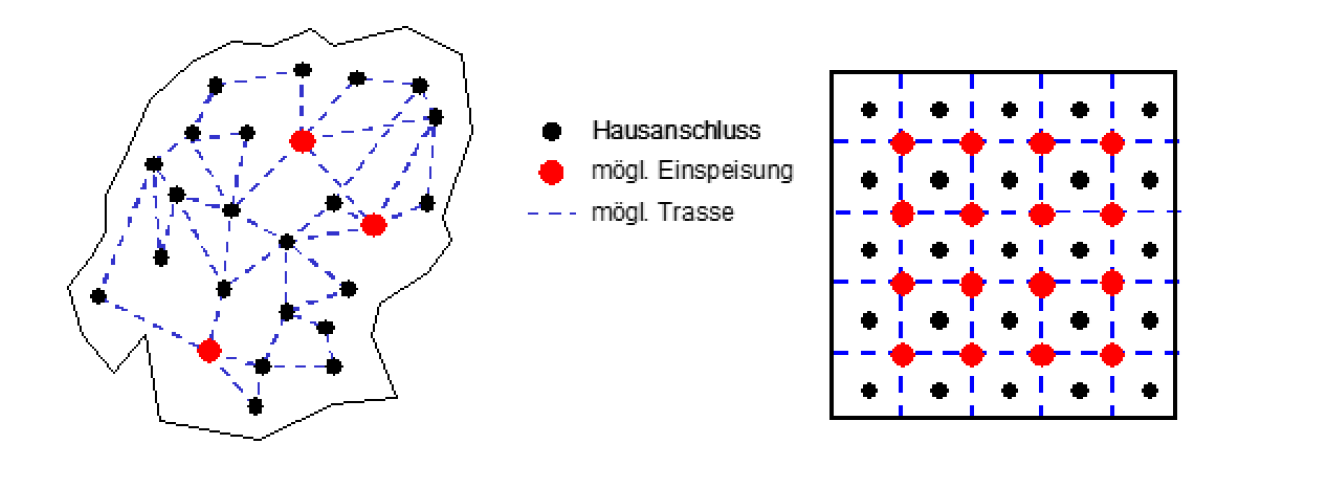
\includegraphics[width=0.8\textwidth]{figures/bfe_ep2050_netz_MNA_notitle.PNG}
\end{figure}
\vspace{-\baselineskip}
\small
\centering
\textit{Comparison between the real (left) and homogeneous model assumed grid
topology \cite{bfe_ep2050_netz2022}} \hyperlink{back}{\beamerreturnbutton{Literature}}

\end{frame}

% =======================================
\begin{frame}{Appendix: Calibrated Random Forest}
\hypertarget{appendix_randomforest_scatterplot}{}
\vspace{-\baselineskip}
\begin{figure}
    \centering
    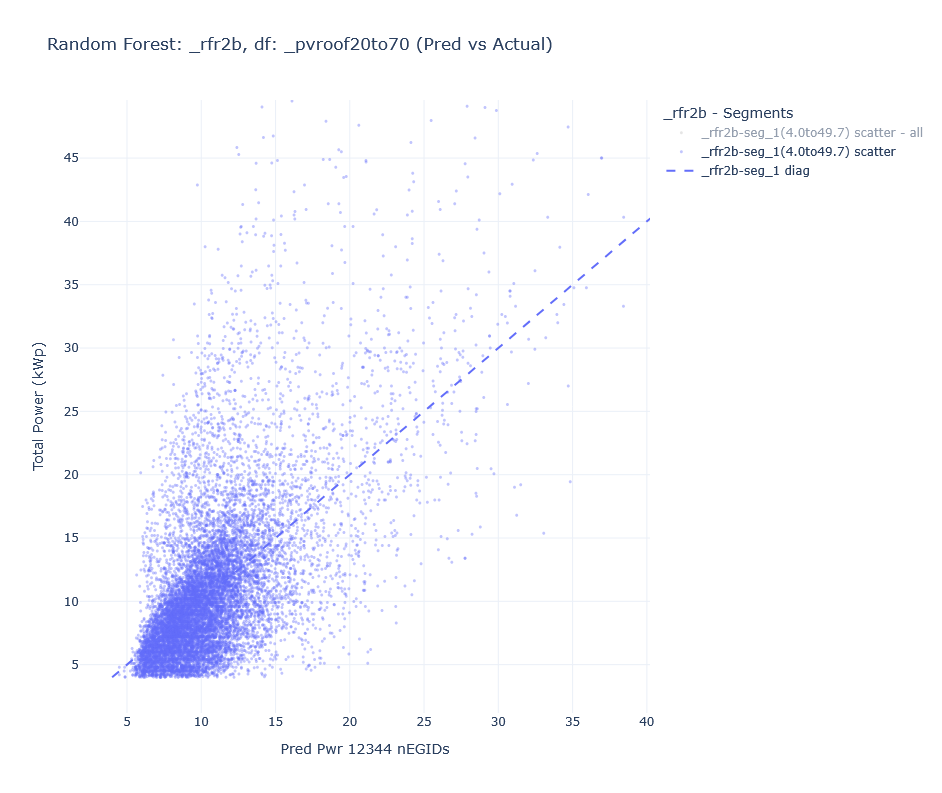
\includegraphics[width=0.6\textwidth]{figures/calib_rfr2_predvsactual.png}
\end{figure}
\vspace{-\baselineskip}
\small
\centering
\textit{Scatterplot for actual and predicted installation sizes (incl 45 degree diagonal) of calibrated random forest regression on 61270 Swiss houses with a PV installation, between 20 to 70 percent an available roof partition used.}\hyperlink{mod_structure_agents}{\beamerreturnbutton{back}}

\end{frame}

% =======================================
\begin{frame}{Appendix: Interpolated Cost Function}
\hypertarget{appendix_cost_function}{}
\vspace{-\baselineskip}
\begin{figure}
    \centering
    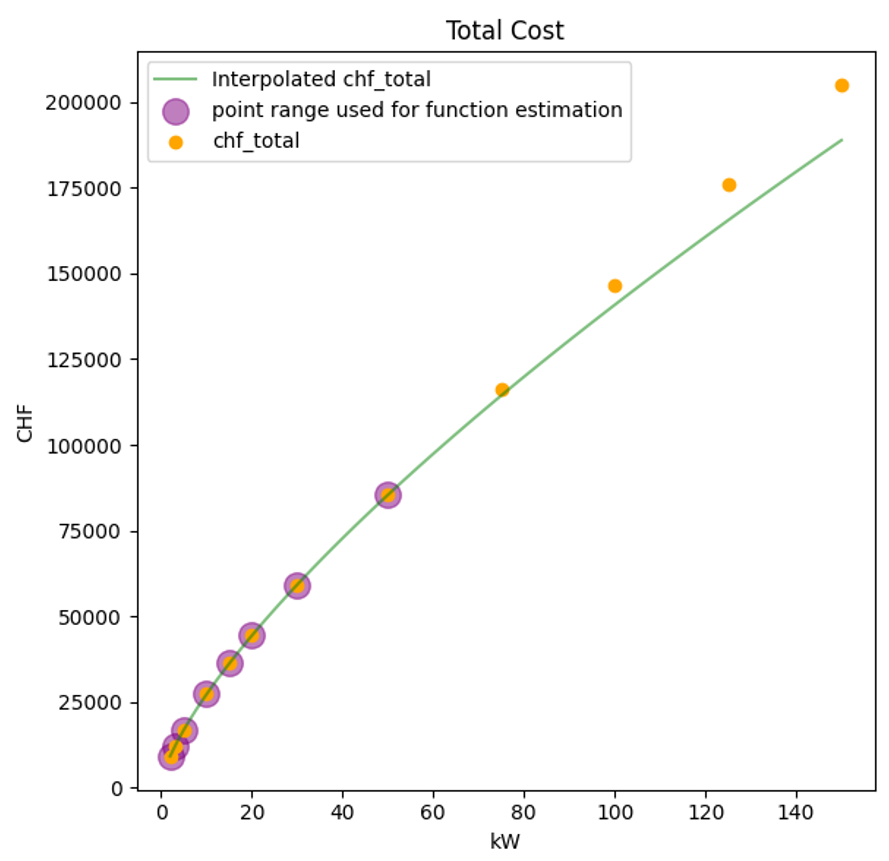
\includegraphics[width=0.6\textwidth]{figures/pvinstcost_table.png}
\end{figure}
\vspace{-\baselineskip}
\small
\centering
\textit{Intrapolation approximation function (green, only on small scale installations) based on
cost assumptions in the technical model appendix of energieschweiz.}\hyperlink{mod_structure_agents}{\beamerreturnbutton{back}}

\end{frame}

% =======================================
\begin{frame}{Appendix: RES Targets 2050 Switzerland}
\hypertarget{appendix_res_targets}{}
\vspace{-\baselineskip}
\begin{figure}
    \centering
    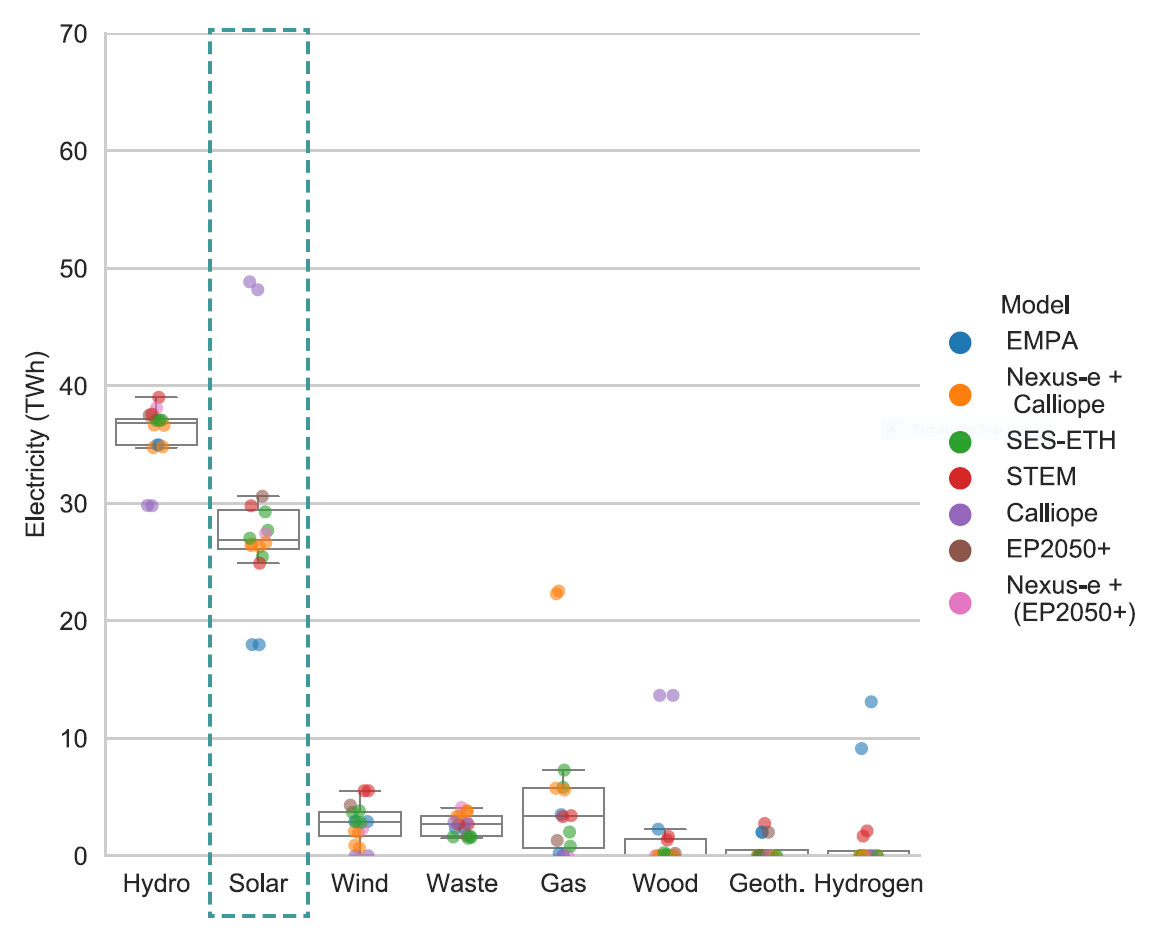
\includegraphics[width=0.7\textwidth]{figures/eth_summerschool_scenario_agg_notitle.png}
\end{figure}
\vspace{-\baselineskip}
\small
\centering
\textit{}\hyperlink{motivation_relevance}{\beamerreturnbutton{back}}
\end{frame}



%%%%%%%%%%%%%%%%%%%%%%%%%%%%%%%%%%%%%%%%%%%%%%

% =======================================
\renewcommand{\bibfont}{\footnotesize}
\begin{frame}[allowframebreaks]{References}
\printbibliography

\end{frame}
\end{document}
